\section{解析函数的幂级数表示}

复级数的收敛性:
\[
\sum_{n=1}^{\infty} \lvert c _n \rvert \text{收敛}\implies \sum_{n=1}^{\infty} c _n\text{收敛}
\]
收敛半径:
\[
\limsup_{ n \to \infty } \sqrt[n]{ \lvert c_n \rvert  }=\frac{1}{R}
\]
解析函数的泰勒展开式:
\[
f(z)=\sum_{n=0}^{\infty} c_n(z-a)^{n}
\]
\[
c_n=\frac{1}{2\pi i}\oint_{C_{\epsilon}} \frac{f(\zeta)}{(\zeta-a)^{n+1}} \, \mathrm{d}\zeta=\frac{f^{(n)}(a)}{n!}
\]
\[
[\ln(1+z)]_{k}=2k\pi i+z-\frac{z^2}{2}+\frac{z^{3}}{3}+\dots+(-1)^{n-1}\frac{z^{n}}{n}+\dots
\]
\subsection{用间接法展开为幂级数}

\begin{exercise}
求 $f(z)=e^{ z }\cos z$ 在 $z=0$ 的泰勒展开式.
\end{exercise}
因为
\[
e^{ z }\cos z=\frac{1}{2}e^{ z }(e^{ iz }+e^{ -iz })=\frac{1}{2}[e^{ (1+i)z }+e^{ (1-i)z }]
\]
于是
\[
e^{ z }\cos z=\frac{1}{2}\left[ \sum_{n=0}^{\infty} \frac{\overbrace{ (1+i)^{n} }^{ (\sqrt{ 2 })^{n}e^{ n\pi i/4 } }}{n!}z^{n}+\sum_{n=0}^{\infty} \frac{\overbrace{ (1-i)^{n} }^{ (\sqrt{ 2 })^{n}e^{ -n\pi i/4 } }}{n!}z^{n} \right]=\sum_{n=0}^{\infty} \frac{(\sqrt{ 2 })^{n}\cos\frac{n\pi }{4}}{n!}z^{n}
\]
\begin{figure}[H]
\centering
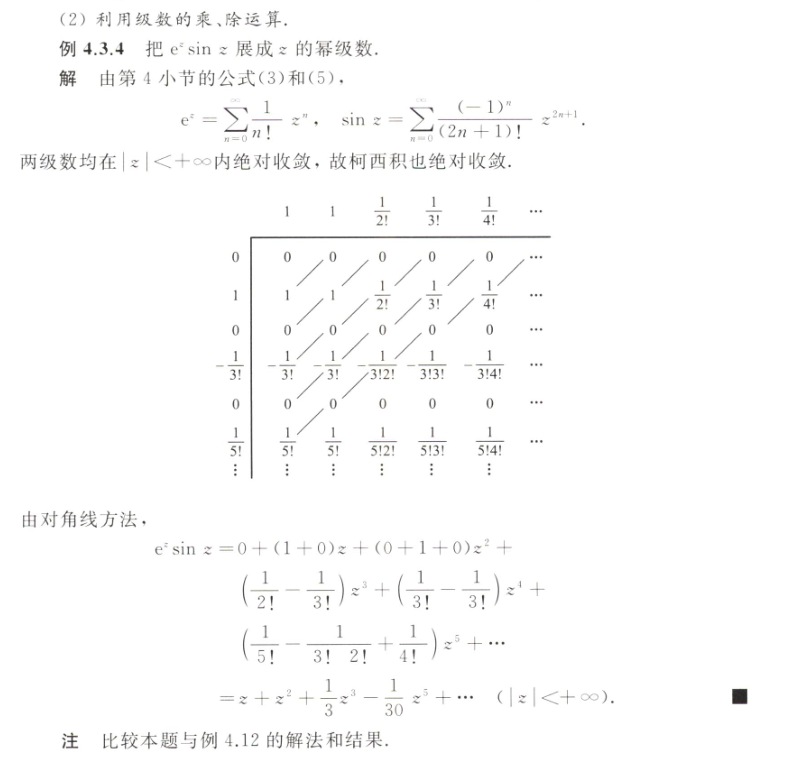
\includegraphics[width=\textwidth]{解析函数的幂级数表示-2025040611.png}
% \caption{}
\label{}
\end{figure}

\begin{exercise}
求 $\tan z$ 在 $z=0$ 的泰勒展式.
\end{exercise}
通过分析奇点可知,$\tan z$ 在 $\lvert z \rvert<\frac{\pi}{2}$ 内解析. 利用“大除法”:

\begin{figure}[H]
\centering
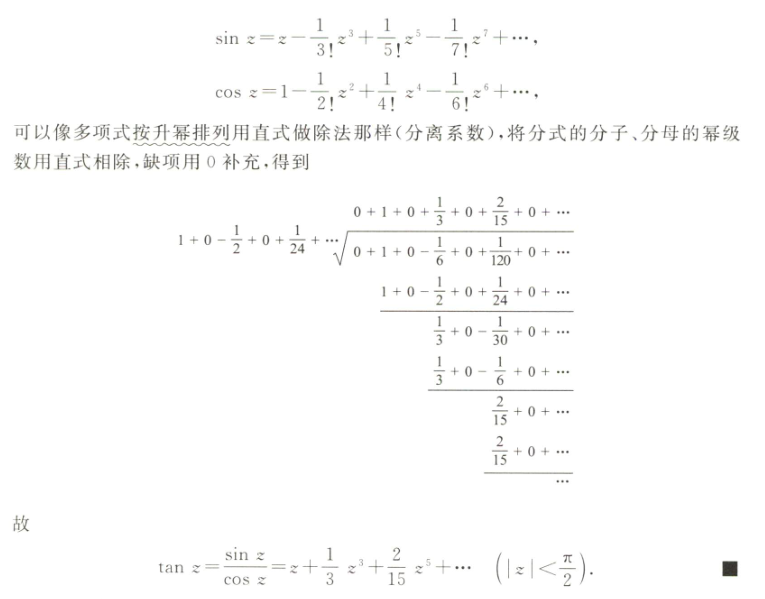
\includegraphics[width=\textwidth]{1-解析函数的幂级数表示-2025040611.png}
% \caption{}
\label{}
\end{figure}

\subsection{待定系数法展开幂级数}

\begin{exercise}
求 $\sec z$ 在 $z=0$ 的泰勒展式.
\end{exercise}
\begin{figure}[H]
\centering
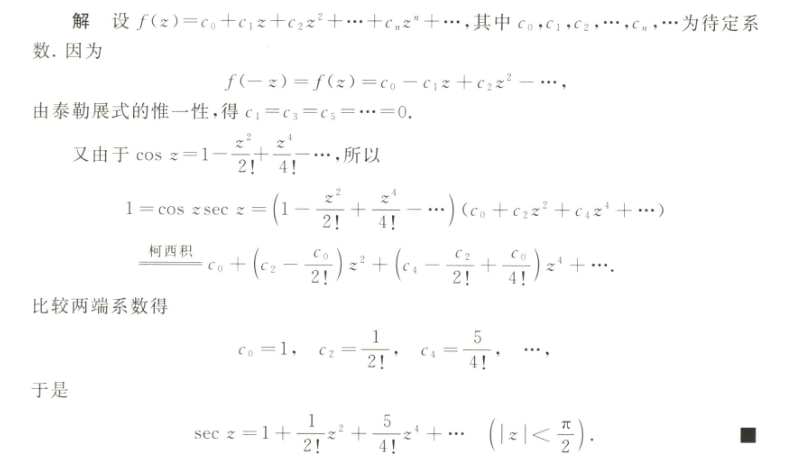
\includegraphics[width=\textwidth]{2-解析函数的幂级数表示-2025040611.png}
% \caption{}
\label{}
\end{figure}

\subsection{微分方程法}

\begin{exercise}
展开 $e^{ 1/(1-z) }$.
\end{exercise}
\begin{figure}[H]
\centering
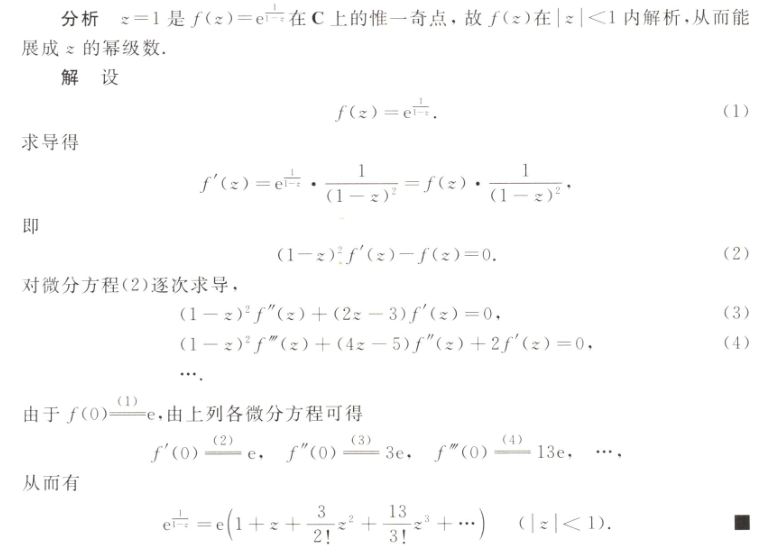
\includegraphics[width=\textwidth]{3-解析函数的幂级数表示-2025040611.png}
% \caption{}
\label{}
\end{figure}

\subsection{逐项求导法}

\begin{figure}[H]
\centering
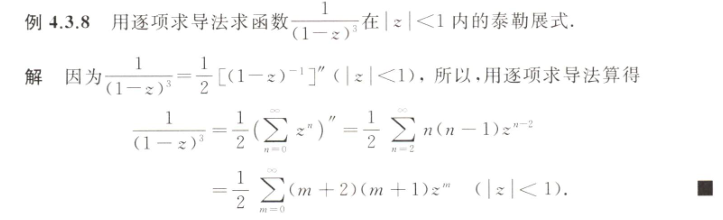
\includegraphics[width=\textwidth]{4-解析函数的幂级数表示-2025040611.png}
% \caption{}
\label{}
\end{figure}

\subsection{逐项积分法}

\begin{figure}[H]
\centering
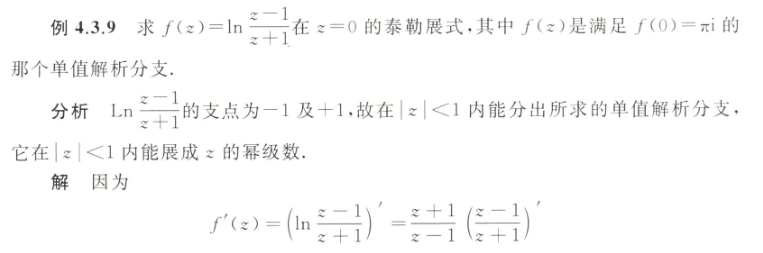
\includegraphics[width=\textwidth]{5-解析函数的幂级数表示-2025040611.png}
% \caption{}
\label{}
\end{figure}
\begin{figure}[H]
\centering
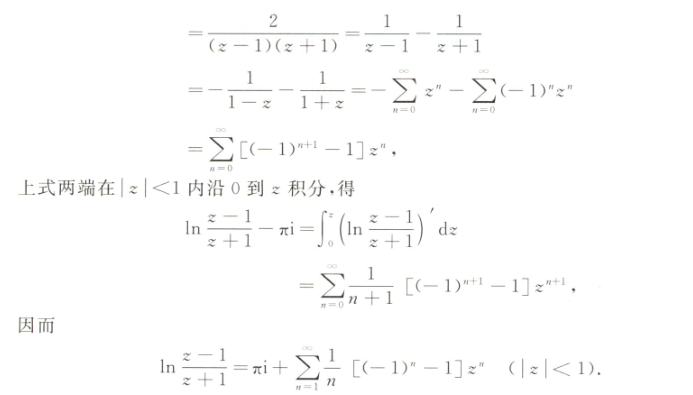
\includegraphics[width=\textwidth]{6-解析函数的幂级数表示-2025040611.png}
% \caption{}
\label{}
\end{figure}

\begin{figure}[H]
\centering
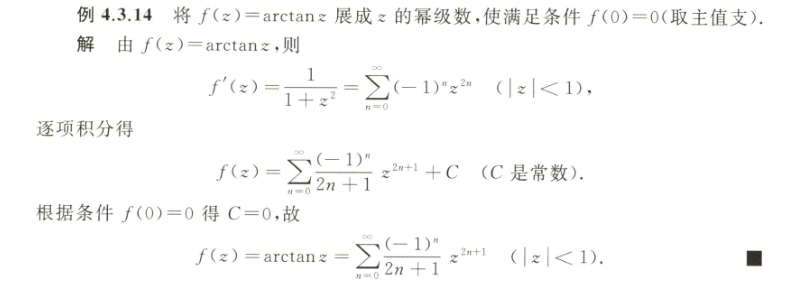
\includegraphics[width=\textwidth]{7-解析函数的幂级数表示-2025040611.png}
% \caption{}
\label{}
\end{figure}

\section{通过幂级数法来证明不等式}

\begin{exercise}
若 $1+w=(1-a)e^{ a }$,且 $\lvert a \rvert<1$,则
\[
\lvert w \rvert \leq \frac{\lvert a \rvert ^2}{1-\lvert a \rvert }
\]
\end{exercise}
\begin{proof}
因为
\[
\begin{aligned}
(1-a)e^{ a }&= (1-a)\left( 1+a+\frac{a^2}{2!}+\dots+\frac{a^{n}}{n!}+\dots \right) \\
 & =1+a+\frac{1}{2!}a^2+\dots+\frac{a^{n}}{n!}+\dots-a-a^2-\dots-\frac{a^{n}}{(n-1)!}-\dots \\
 & =1-\frac{a^2}{2}-\left( 1-\frac{1}{n} \right)\frac{a^{n}}{(n-1)!}-\dots \quad (\lvert a \rvert <1) 
\end{aligned}
\]
所以
\[
\begin{aligned}
\lvert (1-a)e^{a}-1 \rvert  & =\lvert w \rvert \leq \frac{\lvert a \rvert ^{2}}{2}+\dots+\frac{n-1}{n!}\lvert a \rvert ^{n}+\dots \\
 & =\lvert a \rvert ^2+\lvert a \rvert ^{3}+\dots+\lvert a \rvert ^{n}+\dots \\
 & =\frac{\lvert a \rvert ^2}{1-\lvert a \rvert }
\end{aligned}
\]
\end{proof}
\begin{figure}[H]
\centering
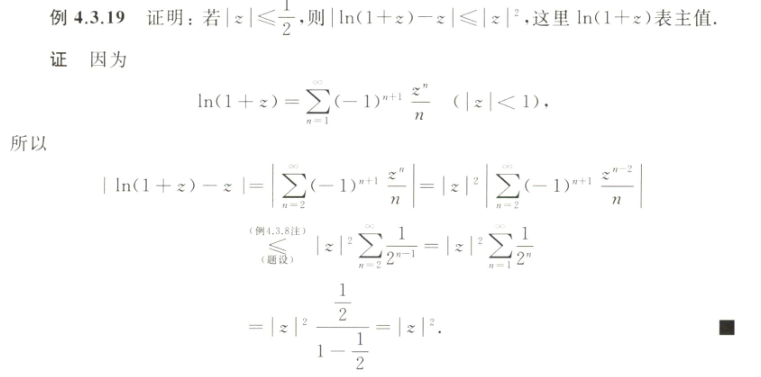
\includegraphics[width=\textwidth]{8-解析函数的幂级数表示-2025040611.png}
% \caption{}
\label{}
\end{figure}

\begin{figure}[H]
\centering
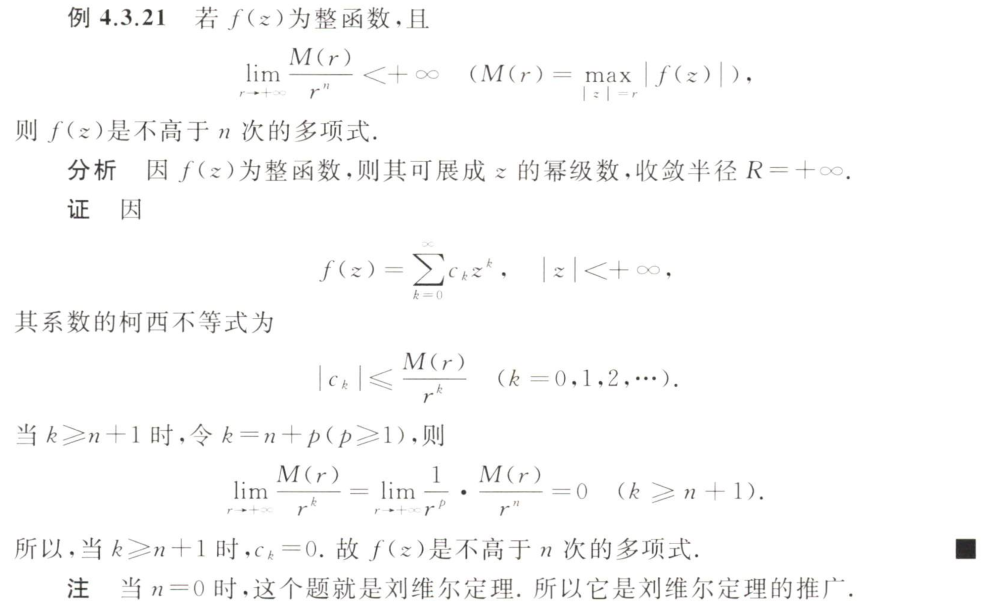
\includegraphics[width=\textwidth]{9-解析函数的幂级数表示-2025040611.png}
% \caption{}
\label{}
\end{figure}

\subsection{最大模定理的应用}

\begin{figure}[H]
\centering
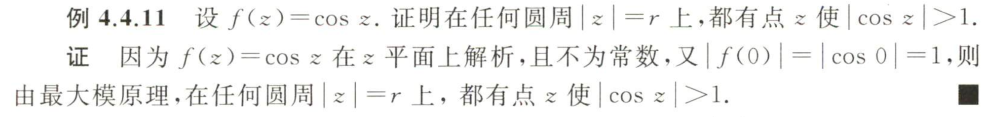
\includegraphics[width=\textwidth]{10-解析函数的幂级数表示-2025040611.png}
% \caption{}
\label{}
\end{figure}

\begin{figure}[H]
\centering
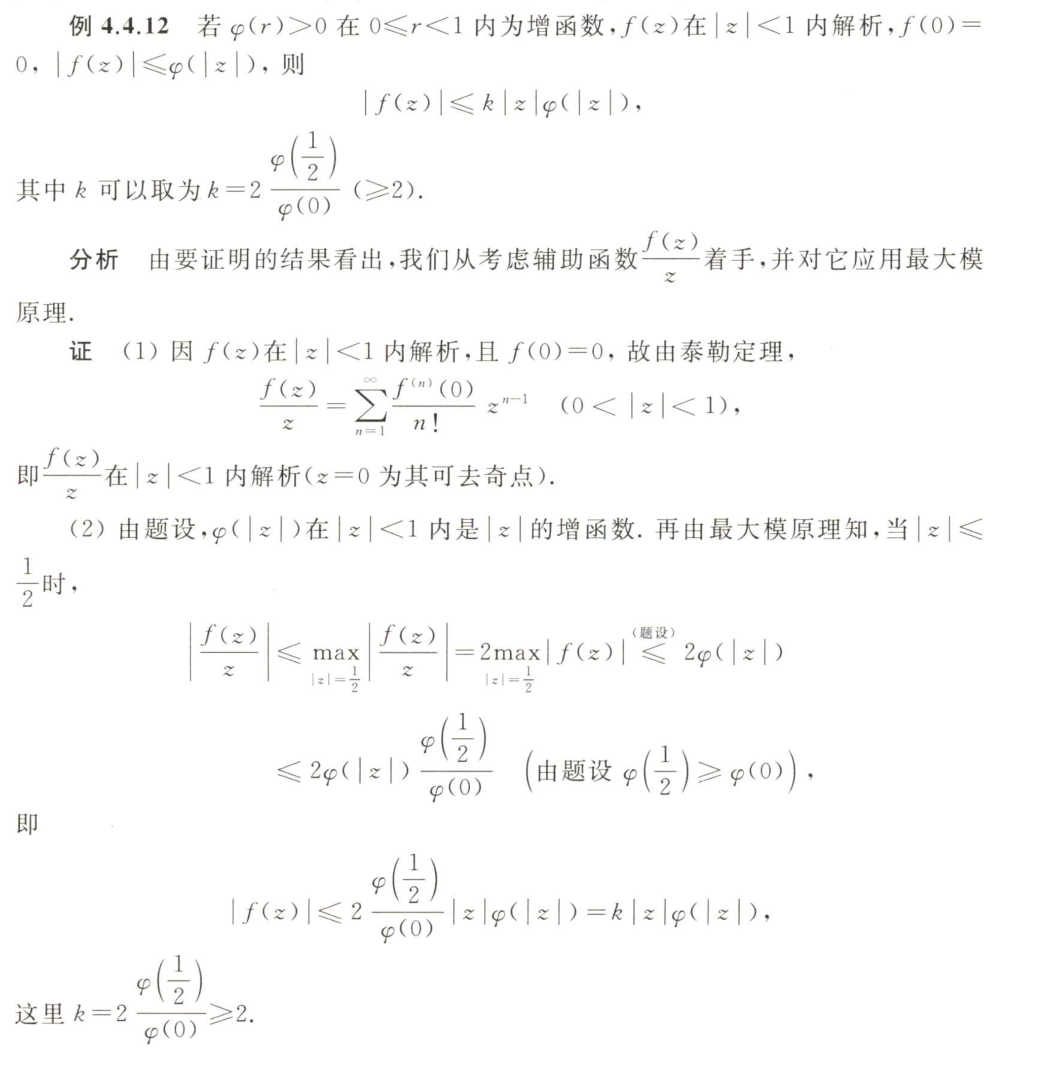
\includegraphics[width=\textwidth]{11-解析函数的幂级数表示-2025040611.png}
% \caption{}
\label{}
\end{figure}
\begin{figure}[H]
\centering
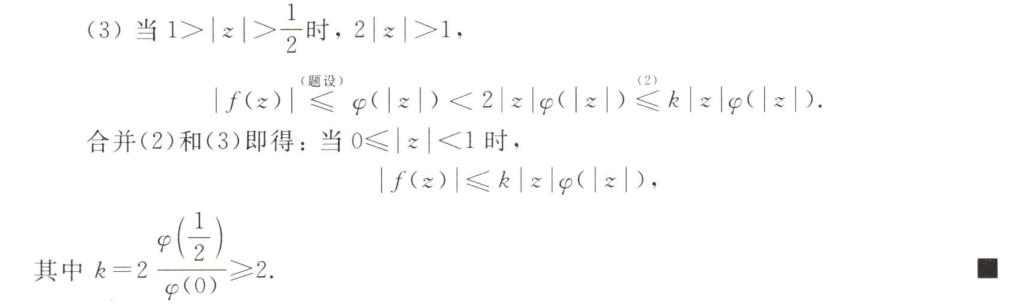
\includegraphics[width=\textwidth]{12-解析函数的幂级数表示-2025040611.png}
% \caption{}
\label{}
\end{figure}

\begin{figure}[H]
\centering
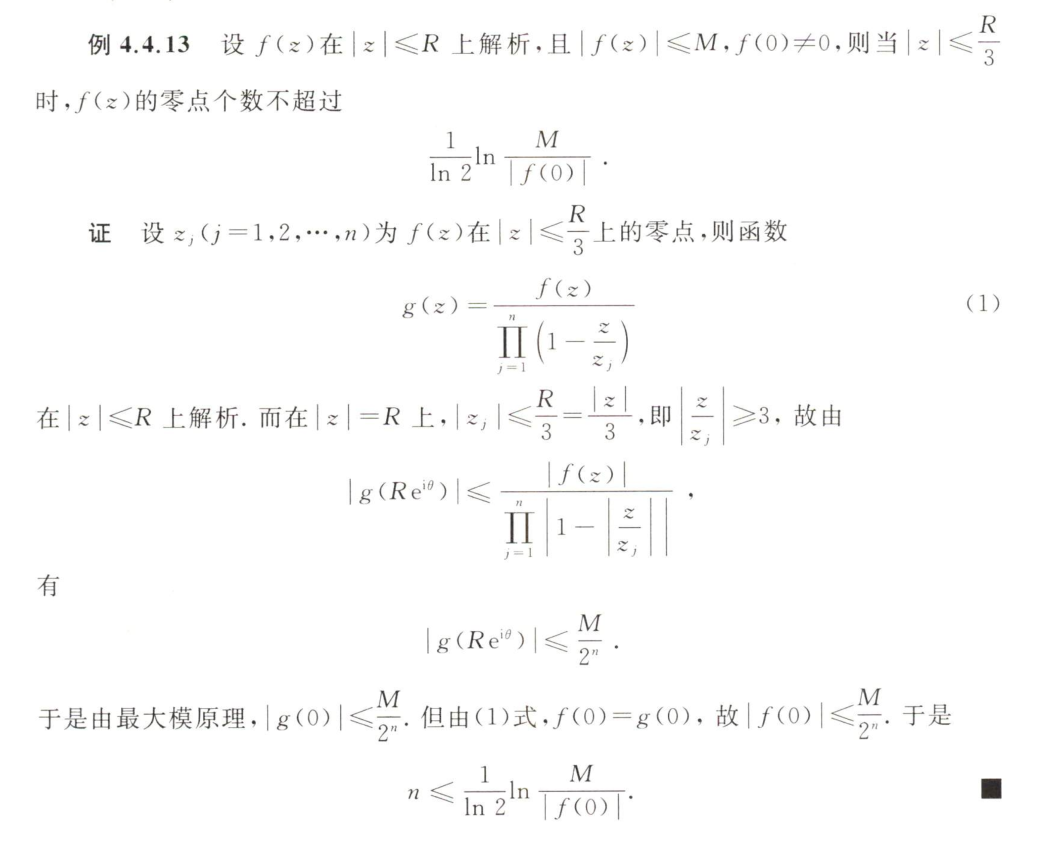
\includegraphics[width=\textwidth]{13-解析函数的幂级数表示-2025040611.png}
% \caption{}
\label{}
\end{figure}

\begin{figure}[H]
\centering
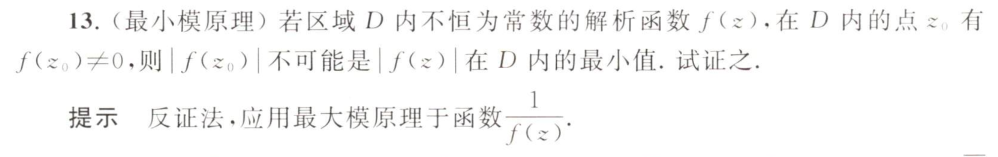
\includegraphics[width=\textwidth]{14-解析函数的幂级数表示-2025040611.png}
% \caption{}
\label{}
\end{figure}

\section{一些习题}

\begin{figure}[H]
\centering
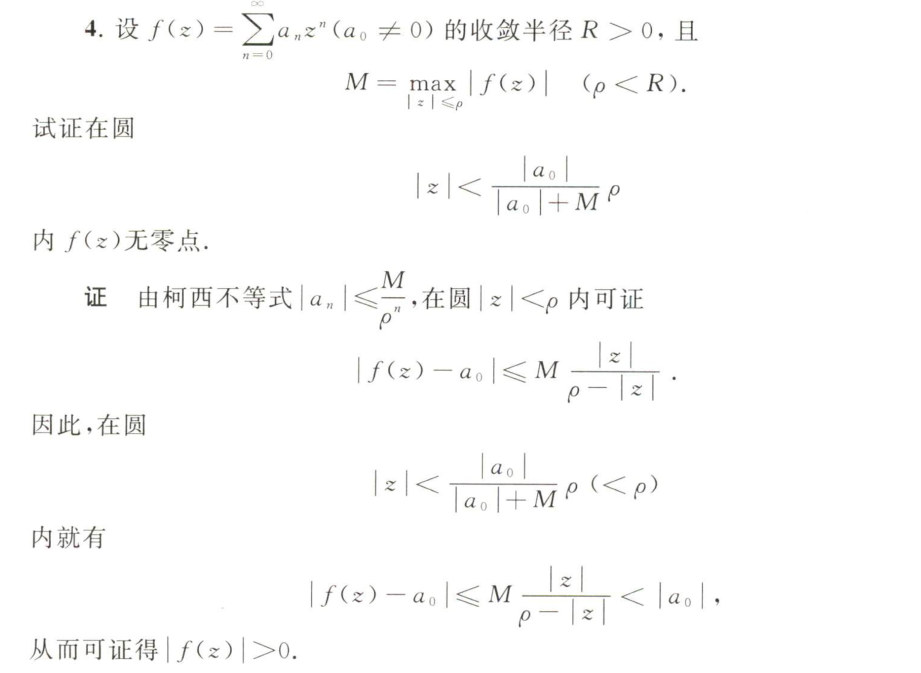
\includegraphics[width=\textwidth]{解析函数的幂级数表示-2025040612.png}
% \caption{}
\label{}
\end{figure}

\begin{exercise}
设函数列 $\{ f_n(z) \}$ 在区域 $G$ 上解析,且在 $G$ 中内闭一致收敛于函数 $f(z)$. 证明:
	\begin{enumerate}
		\item 若 $f(z)$ 不恒为零,$l$ 是 $G$ 内可求长的简单闭曲线,其内部属于 $G$ ,且不经过 $f(z)$ 的零点,则存在正整数 $N$, 使得当 $n\geq N$ 时,在 $l$ 的内部 $f_n(z)$ 和 $f(z)$ 有相同个数的零点.
		\item 若 $\{ f_n(z) \}$ 在区域 $G$ 内部时单叶的,$f(z)$ 不为常数,则 $f(z)$ 在 $G$ 内单叶解析.
	\end{enumerate}
\end{exercise}
\begin{proof}
由 Weierstrass 定理,$f(z)$ 在 $G$ 内解析. 因为 $f(z)$ 在 $l$ 上不为零,则
\[
\min_{z\in l}\lvert f(z) \rvert =m>0.
\]
又 $\{ f_n(z) \}$ 在 $l$ 上一致收敛到 $f(z)$,存在正整数 $N$,使得当 $n\geq N$ 时,在 $l$ 上有 $\lvert f(z)-f_n(z) \rvert<m$. 即当 $n\geq N$ 时,在 $l$ 上有 $\lvert f(z)-f_n(z) \rvert<\lvert f(z) \rvert$. 由 Rouche 定理,在 $l$ 的内部,$f_n(z)$ 和 $f(z)$ 有相同个数的零点.

对于第二问采用反证法,若 $f$ 在 $G$ 内不是单叶的,则存在 $z_1\neq z_2$ 使得 $f(z_1)=f(z_2)$,考虑函数 $g(z)=f(z)-f(z_1)$,圆周 $C_{\epsilon}(z_1),C_{\epsilon}(z_2)$,其中 $\epsilon$ 充分小使得其包含于 $G$ 内,而且 $g(z)$ 在圆周内有唯一的零点. 于是存在 $N$ ,使得 $n\geq N$ 时,$f_n(z)$ 和 $f(z)$ 在 $C_{\epsilon}(z_1),C_{\epsilon}(z_2)$ 内有相同个数(1 个)零点 $z_1^{*},z_2^{*}$,从而 $f_n(z_2^{*})=f(z_1)=f_n(z_1^{*})$. 这与 $f_n$ 的单叶性矛盾!
\end{proof}

\begin{exercise}[cmc 高年级第 10 届]
设 $z_0$ 是复函数 $w=f(z)$ 的 $n$ 阶极点. 证明:一定存在 $\rho>0,R>0$ 使得对于任意 $w\in \{ w\in \mathbb{C}:\lvert w \rvert>R \}$,函数 $f(z)-w$ 在 $\lvert z-z_0 \rvert<\rho$ 中必有 $n$ 个零点.
\end{exercise}
\begin{proof}
定义
\[
\varphi(z)=(z-z_0)^{n}f(z)
\]
且在 $z_0$ 处补充定义(因为是可去奇点),于是 $\varphi$ 在 $z_0$ 的一个小邻域内解析,故存在 $\rho>0$ 使得 $\varphi\in H(B_{\rho}(z_0))$. 再令
\[
R\coloneqq \max_{\lvert z-z_0 \rvert =\rho}\left\lvert  \frac{\varphi(z)}{(z-z_0)^{n}}  \right\rvert
\]
由最大模原理,对于 $\lvert z-z_0 \rvert<\rho$ 有
\[
\lvert \varphi(z)(z-z_0)^{-n} \rvert\leq R<\lvert w \rvert  \implies \lvert \varphi (z) \rvert< \lvert w(z-z_0)^{n} \rvert
\]
由 Rouche 定理,函数 $F(z)\coloneqq\varphi(z)-w(z-z_0)^{n}$ 在 $\lvert z-z_0 \rvert <\rho$ 内零点个数与函数 $w(z-z_0)^{n}$ 相等,即为 $n$ 个. 由于 $n$ 是 $f$ 在 $z_0$ 处的极点阶数,故 $\varphi(z_0)\neq0$,于是 $F(z_0)\neq0$. 故 $F(z)$ 在 $0<\lvert z-z_0 \rvert<\rho$ 存在 $n$ 个零点,故 $f(z)-w=\frac{F(z)}{(z-z_0)^{n}}$ 在 $\lvert z-z_0 \rvert <\rho$ 中必有 $n$ 个零点.
\end{proof}

\begin{theorem}[Picard's Big Theorem]
Let $f$ be an analytic function on a punctured neighborhood of $w_{0}$, say on $D=\left\{z: 0<\left|z-w_{0}\right|<r\right\}$.
If $f$ has an essential singularity at $w_{0}$, then $f$ takes on all possible complex values, with at most a single exception, infinitely often in any neighborhood of $w_{0}$.
\end{theorem}
\begin{theorem}[Picard's Little Theorem]
If $f : \mathbb{C} \to \mathbb{C}$ is an entire function which is not constant, then the image of $f$ is either the whole complex plane or the complex plane minus a single point.
\end{theorem}